\documentclass{article}
\usepackage[utf8]{inputenc}

\usepackage{amsthm}
\usepackage{amsfonts}
\usepackage{amsmath}
\usepackage{amssymb}
\usepackage{fullpage}
\usepackage{graphicx}
\usepackage[usenames]{color}
\usepackage{hyperref}
  \hypersetup{
    colorlinks = true,
    urlcolor = blue,       % color of external links using \href
    linkcolor= blue,       % color of internal links 
    citecolor= blue,       % color of links to bibliography
    filecolor= blue,        % color of file links
    }
    
\usepackage{listings}

\definecolor{dkgreen}{rgb}{0,0.6,0}
\definecolor{gray}{rgb}{0.5,0.5,0.5}
\definecolor{mauve}{rgb}{0.58,0,0.82}

\lstset{frame=tb,
  language=haskell,
  aboveskip=3mm,
  belowskip=3mm,
  showstringspaces=false,
  columns=flexible,
  basicstyle={\small\ttfamily},
  numbers=none,
  numberstyle=\tiny\color{gray},
  keywordstyle=\color{blue},
  commentstyle=\color{dkgreen},
  stringstyle=\color{mauve},
  breaklines=true,
  breakatwhitespace=true,
  tabsize=3
}

\theoremstyle{theorem} 
   \newtheorem{theorem}{Theorem}[section]
   \newtheorem{corollary}[theorem]{Corollary}
   \newtheorem{lemma}[theorem]{Lemma}
   \newtheorem{proposition}[theorem]{Proposition}
\theoremstyle{definition}
   \newtheorem{definition}[theorem]{Definition}
   \newtheorem{example}[theorem]{Example}
\theoremstyle{remark}    
  \newtheorem{remark}[theorem]{Remark}


\title{CPSC-402 Report}
\author{Stephen White}

\date{\today}

\begin{document}

\maketitle

\begin{abstract}
In short, the goal is to search for all occurrences of a small string within a larger string. We are trying to emulate the text searching abilities of Regular Expressions. 
\end{abstract}

\tableofcontents

\section{Introduction}\label{intro}

My name is Stephen White. I am a Computer Science major with a minor in Business Administration at Chapman University.

\section{Homework}\label{homework}

This section contains the solutions to the homework. 

\subsection{Week 1}

%For most weeks, you will have a subsection that contains your answers.

\subsubsection{Homework 1.1}
The homework discussed in this section can be seen \href{https://hackmd.io/@alexhkurz/rycnvMvgu}{here}.
Part 1 of the homework is exercise 2.2.4 item B. The problem can be found on page 54 of the textbook (page 69 of the pdf).
\newline \newline
The first question is as follows: "Give DFA's accepting the following languages over the alphabet \{0,1\}: The set of all strings with three consecutive 0's (not necessarily at the end)."
\newline\newline
My answer to this question is as follows:\\
Since we know that this DFA's alphabet can only consist of 0's and 1's, and we are searching for three consecutive 0's, looking like this: 000, we can formally defined the DFA as 
\begin{align*}
    \{\omega\ |\ \omega\ is\ of\ the\ form\ x000y\ for\ some\ strings\ x\ and\ y\ consisting\ of\ 0's\ and\ 1's\ only \}
\end{align*}

The following image is a diagram of this DFA showing its states and transitions.\\
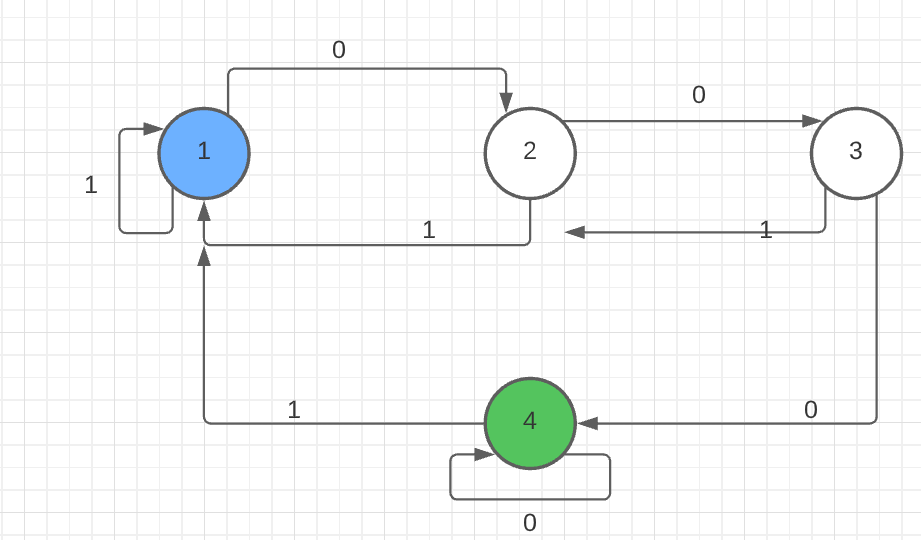
\includegraphics{Question224PartB.png}\\
(I have chosen blue to signify the initial state and green to signify the success state)\\

The next question asks "Give DFA's accepting the following languages over the alphabet \{0,1\}: The set of strings with 011 as a substring."\\\\
My answer to this question is as follows:\\
Since we know that this DFA's alphabet can only consist of 0's and 1's, and we are searching for the string 011, we can formally defined the DFA as 
\begin{align*}
    \{\omega\ |\ \omega\ is\ of\ the\ form\ x011y\ for\ some\ strings\ x\ and\ y\ consisting\ of\ 0's\ and\ 1's\ only \}
\end{align*}

The following image is a diagram of this DFA showing its states and transitions.\\
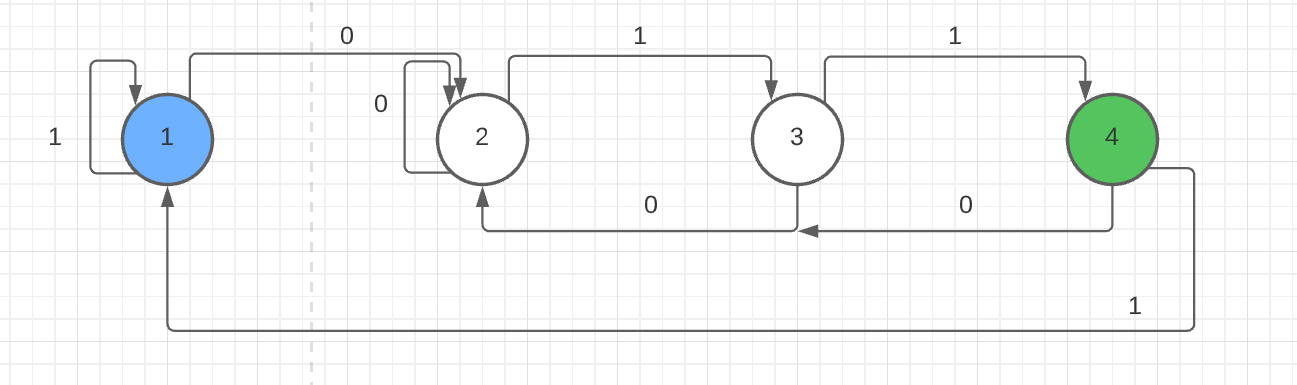
\includegraphics[scale=0.75]{Question224PartC.png}\\
(I have chosen blue to signify the initial state and green to signify the success state)\\

\subsubsection{Homework 1.2}
The homework discussed in this section can be seen \href{https://github.com/alexhkurz/compiler-construction-2022/blob/main/homework-1.2.md}{here}.\\\\

Part 1 of this assignment is to answer the following question: 
\begin{center}
    "Does the file contain the sequence aa or abb? For example, if the file is aaabbaabb, the output should be [2,3,5,7,9]. The challenge here is to not write a program that runs twice through the file, once to search for aa and once for abb, but to find a way of running through the file only once and to simultaneously search for both strings."
\end{center}

I chose to write the program in C\# because I am most familiar with it, and I believe it has a good mix between control and programming speed. That code can be found \href{https://github.com/mamba72/CompilerConstruction_Assignments/blob/main/Reports/ReportResources/StringSearchingImplementation.cs}{here on my GitHub}.
To aid me in my understanding of the problem, I made the following diagram of the DFA I was creating:\\
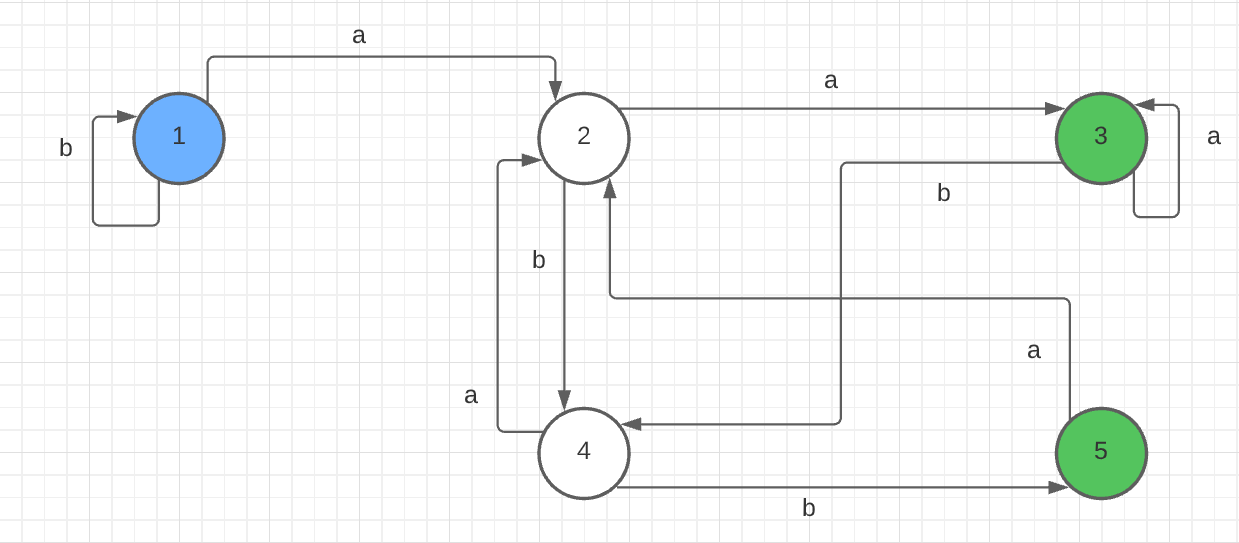
\includegraphics[scale = 0.7]{Question3DFA.png}\\\\

Part 2 of the homework was to complete exercise 2.2.10 (the proof being optional) on page 54 of the textbook (page 70 of the pdf).\\
The question reads as follows:
\begin{center}
    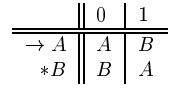
\includegraphics[]{Exercise2210Diagram.png}\\
"Informally describe the language accepted by this DFA."
\end{center}
I tackled this problem by first breaking down the chart, to understand what I was being asked. The chart is similar to a Punnett Square. The left column is a list of the possible current states (an input). The top row is a list of possible character inputs. The rest of the chart is the next state (the output) determined by that row's current state and current character. Since the only possible characters are 1 and 0, the language accepted by this DFA is a set of strings or words created by any combination of 0's and 1's. 


\subsection{Week 2}

\ldots

\section{Project}

The project will be to compile code from a programming language of your choice to assembly and to explain the assembly code and compilation process using the knowledge your learned in this course. 


\medskip\noindent
Pro tips:
\begin{itemize}
\item Choose a compiled (not interpreted) programming language.
\item Choose a language that you find interesting anyway.
\item Start early.
\item Come to office hours. I have not run this part of the course before and I am really interested what you will find.
\end{itemize}
 
\section{Conclusions}\label{conclusions}

%(approx 400 words)

%In the conclusion, I want a critical reflection on the content of the course. Step back from the technical details. How does the course fit into the wider world of programming languages and software engineering?

\begin{thebibliography}{99}
\bibitem[HMU]{Hopcroft}
	John E. Hopcroft, Rajeev Motwani, Jeffrey D. Ullman:
\href{http://ce.sharif.edu/courses/94-95/1/ce414-2/resources/root/Text%20Books/Automata/John%20E.%20Hopcroft,%20Rajeev%20Motwani,%20Jeffrey%20D.%20Ullman-Introduction%20to%20Automata%20Theory,%20Languages,%20and%20Computations-Prentice%20Hall%20(2006).pdf}{Introduction to automata theory, languages, and computation,} 3rd Edition. Pearson international edition, Addison-Wesley 2007

\end{thebibliography}

\end{document}
